\pdfcompresslevel=0
\documentclass{article}
\usepackage{mathptmx}

\usepackage{tikz}


\begin{document}
\fontname\font
\usetikzlibrary{shapes.symbols}
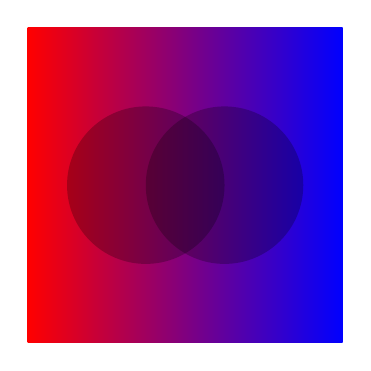
\begin{tikzpicture}
    \shade [left color=red, right color=blue] (3,-2) rectangle (7,2);
        \begin{scope}[opacity=.25, transparency group={isolated=false}]
        \fill[black] (4.5,0) circle (1);
    \end{scope}
    \begin{scope}[opacity=.25, transparency group={isolated=false}]
        \fill[black] (5.5,0) circle (1);
    \end{scope}
\end{tikzpicture}

\end{document}
